\documentclass[tikz,border=5pt]{standalone}
\usepackage{tikz}
\usetikzlibrary{calc,positioning,shapes.misc}
\usepackage{xcolor}

% Definir cores IME
\definecolor{imeblue}{RGB}{20,45,105}
\definecolor{imesoftblue}{RGB}{0,100,160}
\definecolor{imeyellow}{RGB}{230,175,60}
\definecolor{imered}{RGB}{130,20,60}

\begin{document}

% Gráfico de Pizza: Usage of AI tools in development
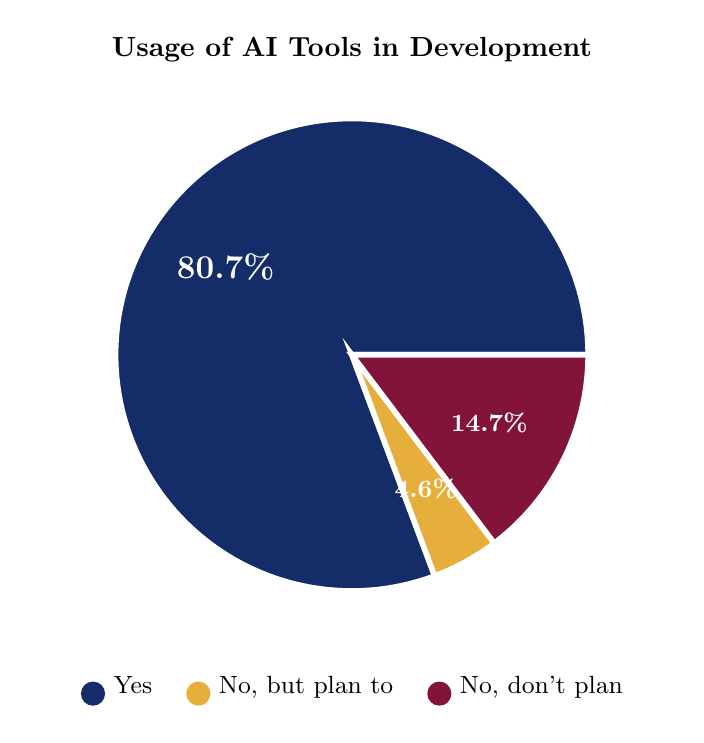
\begin{tikzpicture}[scale=1.2]
  \def\radius{2.5}
  \def\centerx{0}
  \def\centery{0}
  
  % Dados: Yes=80.7%, No but plan=4.6%, No don't plan=14.7%
  % Converte para ângulos: 80.7° × 3.6 = 290.52°, 4.6° × 3.6 = 16.56°, 14.7° × 3.6 = 52.92°
  
  % Slice 1: Yes (80.7%) - imeblue - 0° a 290.52°
  \draw[fill=imeblue, draw=white, line width=2pt] 
    ({\centerx + \radius}, {\centery}) 
    arc (0:290.52:\radius) 
    -- ({\centerx}, {\centery}) 
    -- cycle;
  
  % Slice 2: No, but plan to (4.6%) - imeyellow - 290.52° a 307.08°
  \draw[fill=imeyellow, draw=white, line width=2pt] 
    ({\centerx + \radius*cos(290.52)}, {\centery + \radius*sin(290.52)}) 
    arc (290.52:307.08:\radius) 
    -- ({\centerx}, {\centery}) 
    -- cycle;
  
  % Slice 3: No, don't plan (14.7%) - imered - 307.08° a 360°
  \draw[fill=imered, draw=white, line width=2pt] 
    ({\centerx + \radius*cos(307.08)}, {\centery + \radius*sin(307.08)}) 
    arc (307.08:360:\radius) 
    -- ({\centerx}, {\centery}) 
    -- cycle;
  
  % Labels com percentuais
  % Label 1: Yes 80.7% (ângulo médio: 145.26°)
  \node[font=\bfseries\large, text=white, anchor=center] 
    at ({0.65*\radius*cos(145.26)}, {0.65*\radius*sin(145.26)}) 
    {80.7\%};
  
  % Label 2: No, but plan 4.6% (ângulo médio: 298.8°)
  \node[font=\bfseries\small, text=white, anchor=center] 
    at ({0.65*\radius*cos(298.8)}, {0.65*\radius*sin(298.8)}) 
    {4.6\%};
  
  % Label 3: No, don't plan 14.7% (ângulo médio: 333.54°)
  \node[font=\bfseries\small, text=white, anchor=center] 
    at ({0.65*\radius*cos(333.54)}, {0.65*\radius*sin(333.54)}) 
    {14.7\%};
  
  % Legenda abaixo
  \node[anchor=north, font=\small, text width=8cm, align=center] at (0, {-\radius - 0.8})
    {
      \tikz[baseline=(L1.base)]{\node[fill=imeblue, circle, minimum size=0.3cm] (L1) {};} Yes \quad
      \tikz[baseline=(L2.base)]{\node[fill=imeyellow, circle, minimum size=0.3cm] (L2) {};} No, but plan to \quad
      \tikz[baseline=(L3.base)]{\node[fill=imered, circle, minimum size=0.3cm] (L3) {};} No, don't plan
    };
  
  % Título
  \node[anchor=south, font=\bfseries, align=center] at (0, {\radius + 0.5})
    {Usage of AI Tools in Development};
  
\end{tikzpicture}

\end{document}
